\clearpage
\section{Channel 9 ADC and integrators: 16 November 2026}
The owner moved both USB pairs from physical channel 10 to 9. MOD-DAC outputs
0/1 feed J8 (direct ADC), outputs 2/3 feed J6 (integrator); the four CFD fixtures
remain on channels 9--12. No firmware, gateware, clock profile or SMU changes
were made during these measurements. Actual FPGA build is \texttt{ff2f746c}.

\subsection{ADC transfer and adjacent data lines}
Both banks passed a 257-point differential sweep from -1.2 to +1.2 V at 1 V common
mode (each DAC output 0.4--1.6 V), with integrator amplifiers disabled.
Both ADCs exercised every bit at zero/one and all 44 adjacent-pair states.
This is a functional assembly check, not calibrated INL/DNL or an electrical
proof excluding every possible short.
\begin{center}\begin{tabular}{lrrr}\toprule
ADC & Gain (code/V) & Zero mean (code) & Template-removed RMS (code)\\\midrule
A & -1778.41 & 2168.222 & 0.598 \\
B & -1776.68 & 2171.502 & 0.563 \\
\bottomrule\end{tabular}\end{center}
The residual RMS follows removal of a four-phase template and is not intrinsic
ADC noise or aperture jitter. Voltages are DAC commands, not calibrated readings.
\begin{center}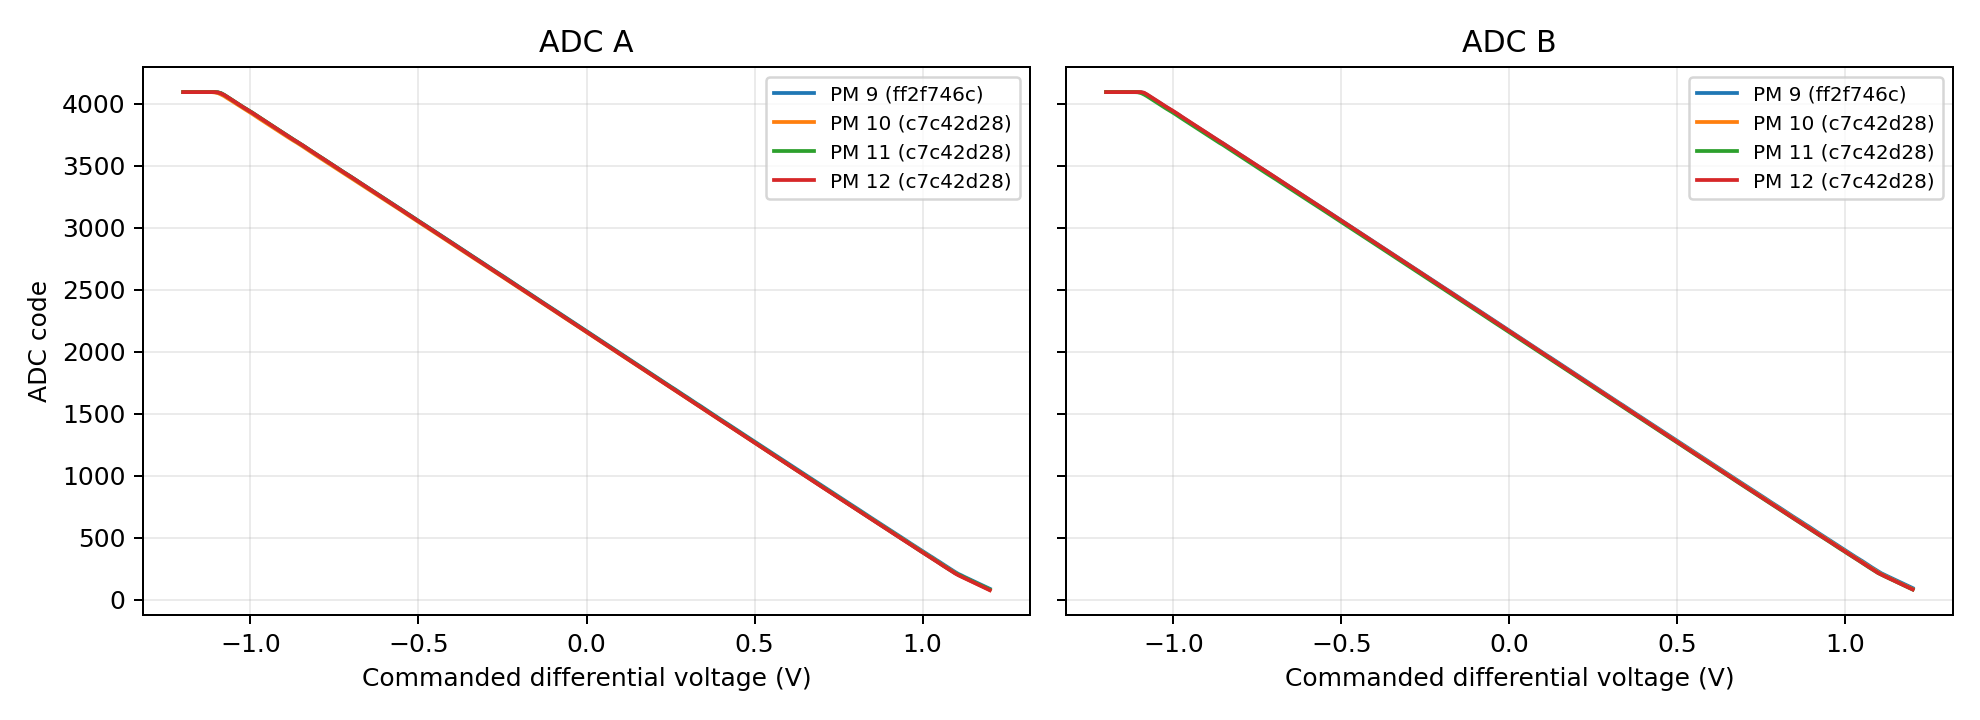
\includegraphics[width=\linewidth]{ch09-adc-response-09-12.png}\end{center}
Channels 10--12 are historical 13 November measurements with build c7c42d28;
channel 9 uses ff2f746c. These are explicitly labelled cross-revision comparisons.
\subsection{Integrator balance and signed response}
Direct ADC injection was inhibited before releasing the integrator amplifiers.
The coordinate is DAC2 = 1.024 V + delta/2, DAC3 = 2.048 V - delta/2.
Coarse13 and fine26 points were followed by independent candidate revisits and
plus/minus5 mV checks. Clipped or ambiguous waveforms are excluded from balance.
\begin{center}\begin{tabular}{lrrr}\toprule
ADC & DAC2/DAC3 (V) & Return change (code) & Gain (code/V)\\\midrule
A & 1.0265/2.0455 & +0.232 & -2543.1 \\
B & 1.0264/2.0456 & -0.050 & -2693.0 \\
\bottomrule\end{tabular}\end{center}
\begin{center}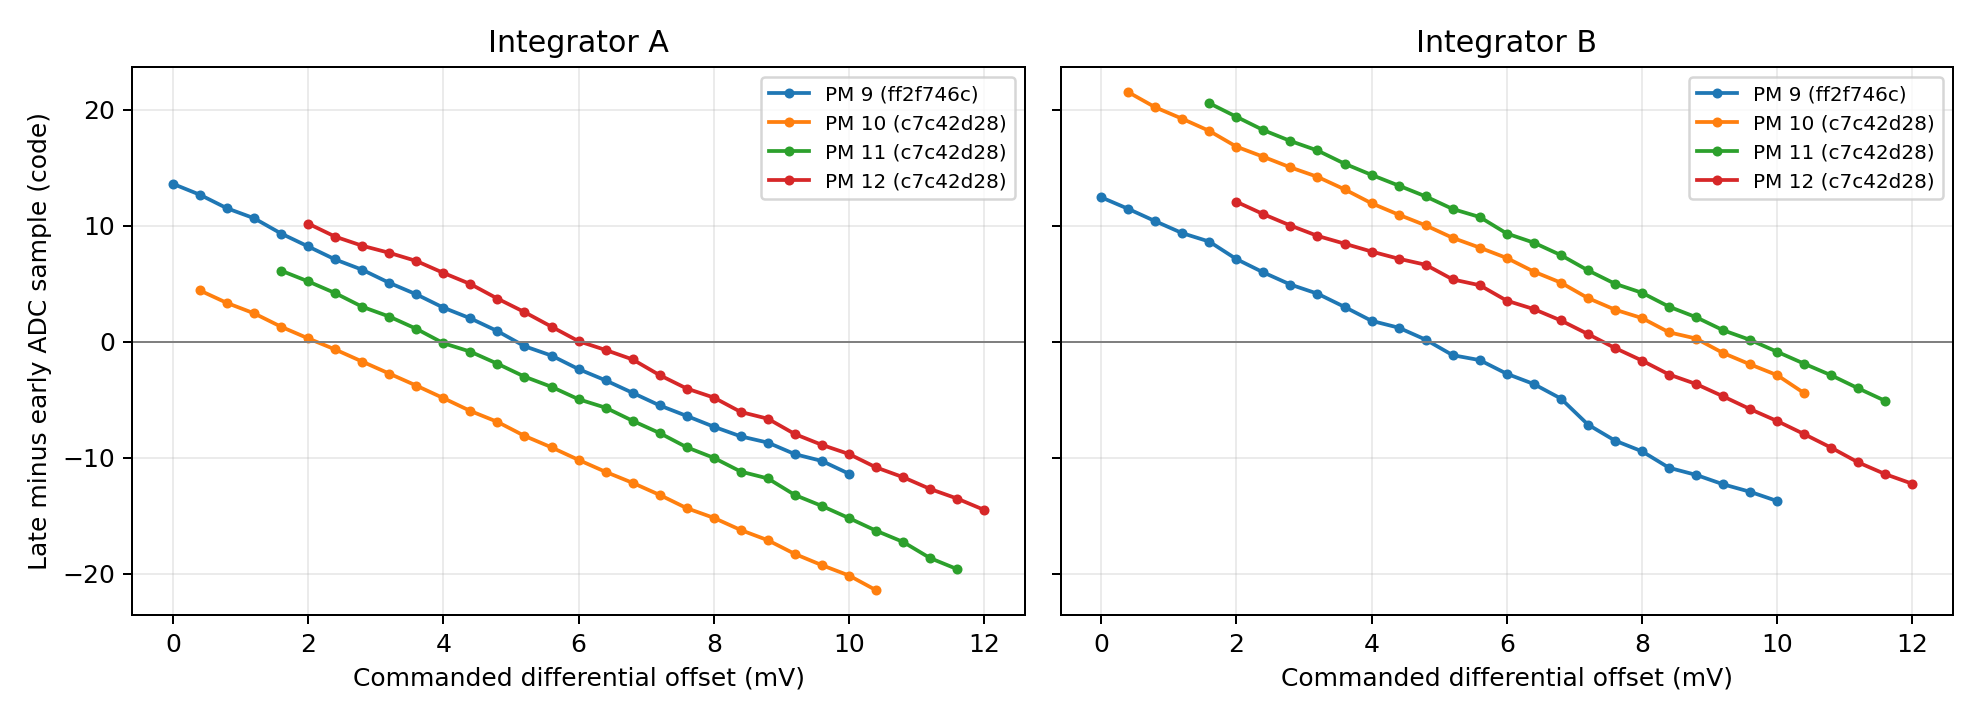
\includegraphics[width=\linewidth]{ch09-integrator-response-09-12.png}\end{center}
\begin{center}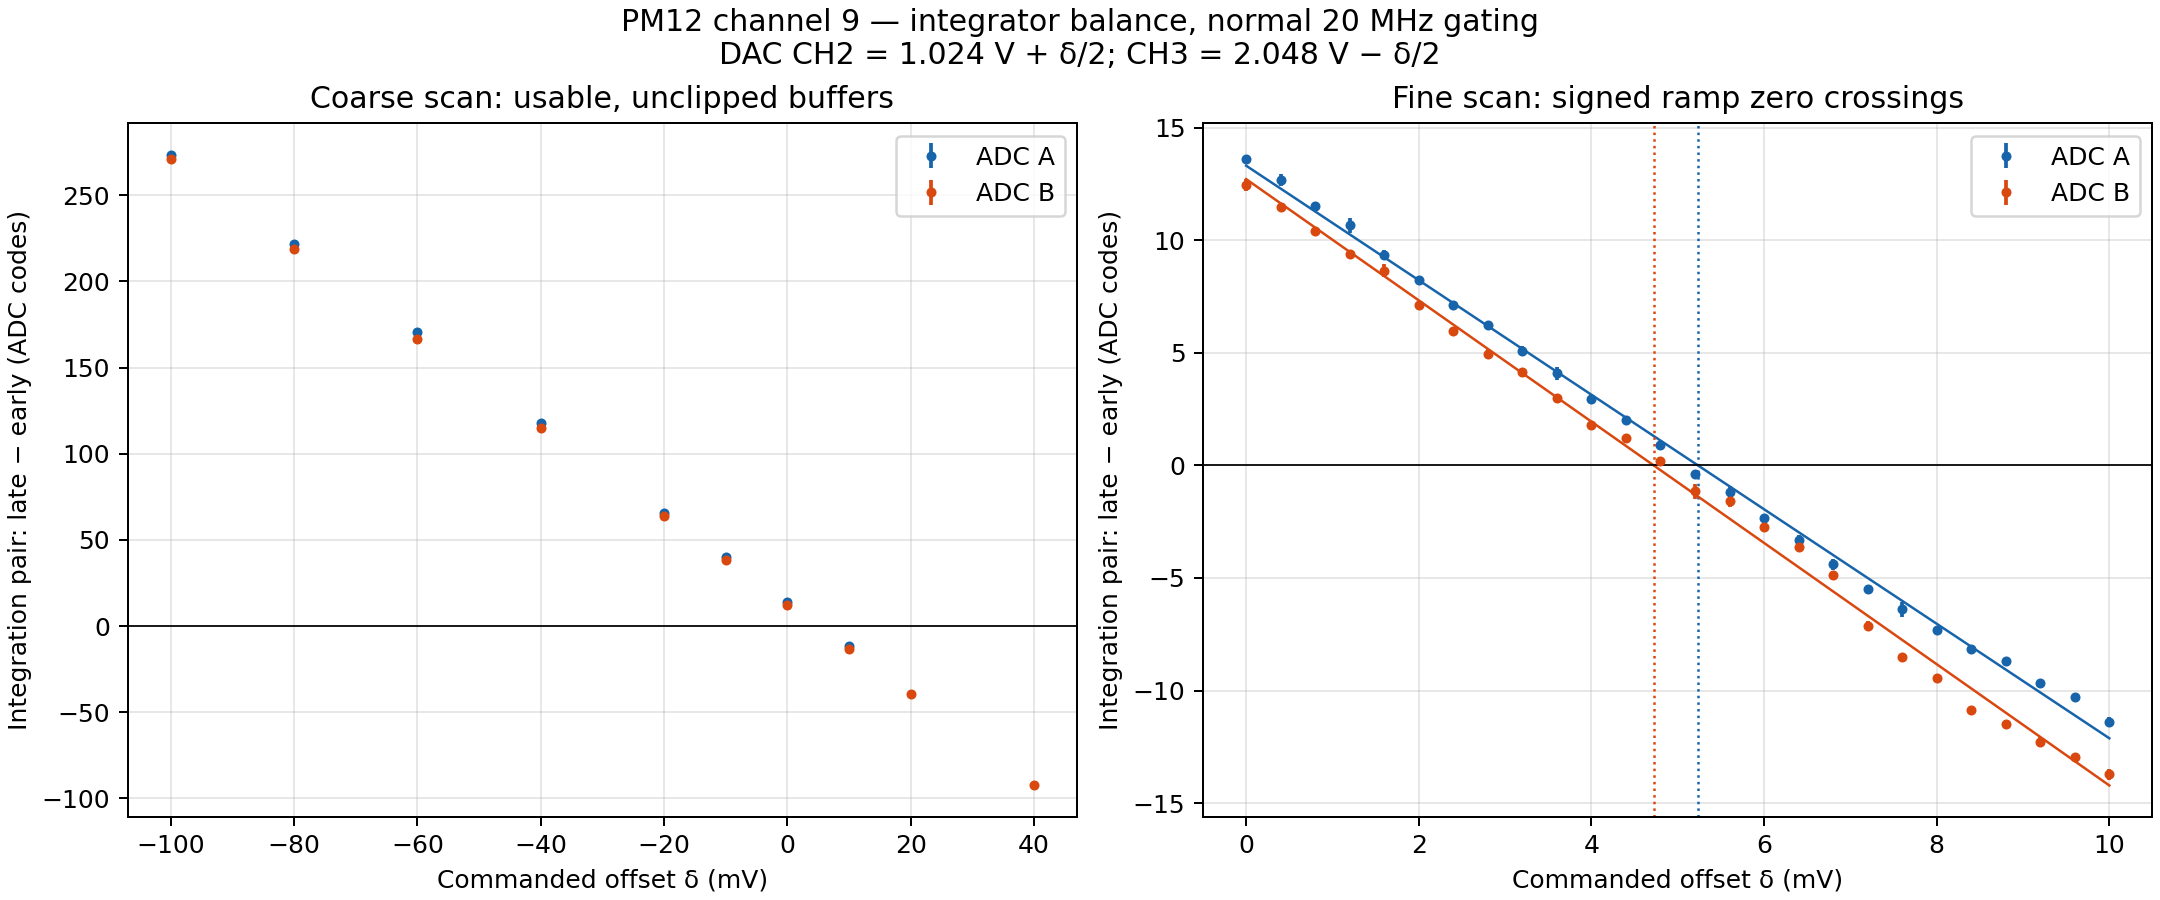
\includegraphics[width=\linewidth]{ch09-integrator-balance.png}\end{center}
\begin{center}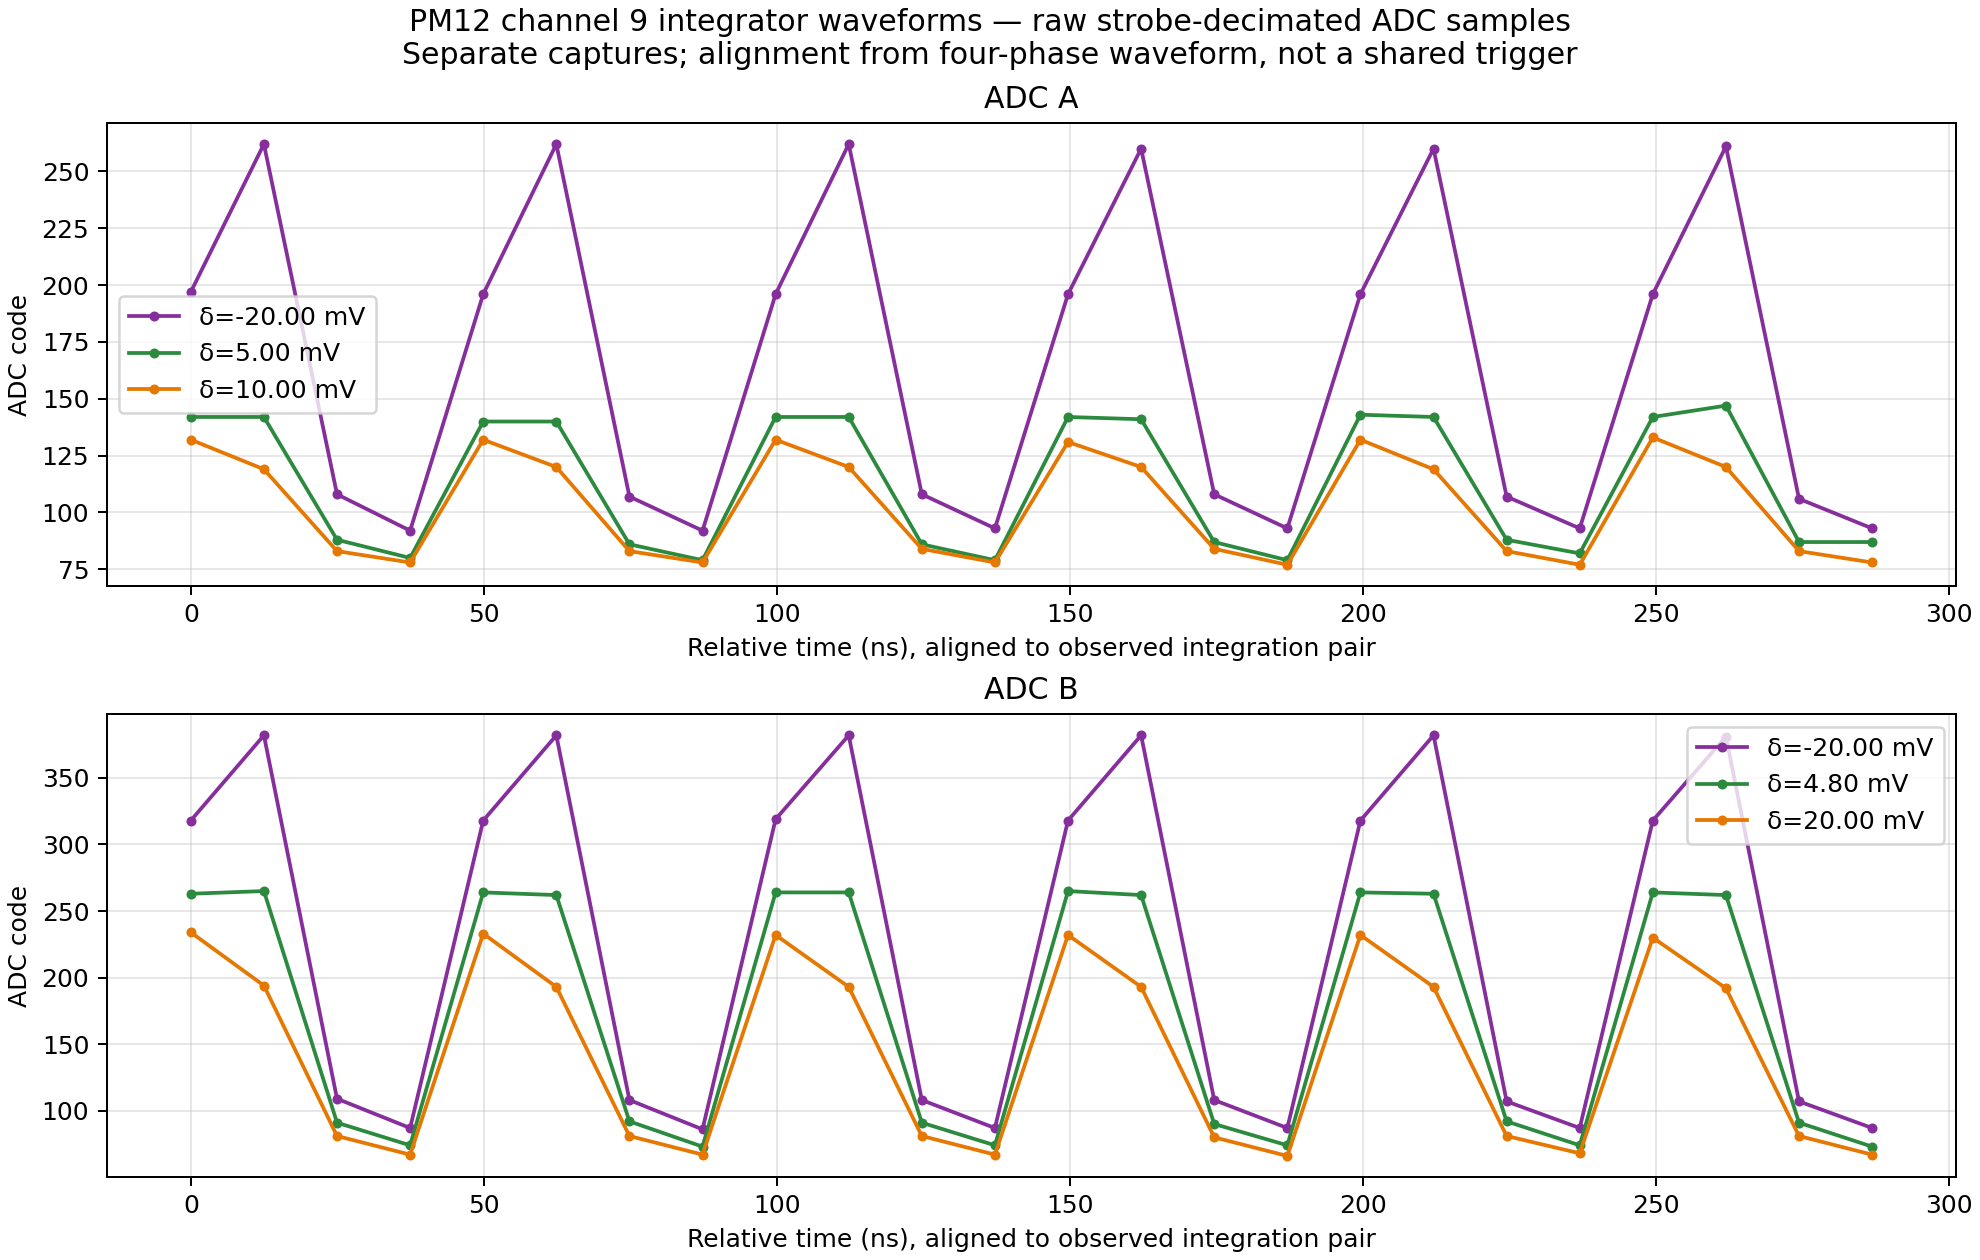
\includegraphics[width=\linewidth]{ch09-integrator-waveforms.png}\end{center}
Waveform pair assignment is not an independently timestamped gate. Balance and
gain include the complete DAC/cable/integrator/ADC chain. Separate A/B balance
points do not imply a shared setting nulls both simultaneously.

\subsection{Provenance and current state}
Analog functional coverage now includes physical channels 9--12, with the
hardware revision distinction above. Prior frozen contracts and results remain
unchanged; the new source/build combination is registered independently.
Both USB pairs remain on9. DAC0/1 are 1/1 V; DAC2/3 are parked at the measured
shared compromise. Channel9 amplifiers enabled, direct ADC injection isolated,
all monitor muxes inhibited and TCA masks zero. Kasli output directions unchanged.
This does not close unrelated board findings or establish full board acceptance.
Raw buffers and editable sources are in the dated channel9 evidence archive.
